\chapter{Opis projektnog zadatka}

		Gubitak kućnog ljubimca može biti jedna od emocionalno najtežih stvari kroz koje vlasnik može proći. Ponekad se dogodi da ljubimac odluta od kuće zbog znatiželje, iznenadnog događaja koji je u njima probudio strah… U tom slučaju, vlasniku je prioritet brzo pronaći mezimca kako bi bio na sigurnom u svom domu.\\
		
		Naša aplikacija je namijenjena onima koji su izgubili kućnog ljubimca, onima koji žele pomoći drugima u pronalasku svojih krznenih prijatelja pa i skloništima koji pod svoje primaju odlutale prestrašene životinje. Svi zainteresirani za dobrobit ovih ljubimaca imaju direktan pristup svim informacijama o njima. Značaj aplikacije za zajednicu je da može doprinijeti smanjenju broja napuštenih ljubimaca i time olakšati rad skloništima za životinje te promovirati svijest o izgubljenim ljubimcima. \\
		
		Ova korisna i jednostavna responzivna aplikacija pomoći će u rješavanju ovog problema mnogim korisnicima aplikacije.\\
		
		Cilj ovog projekta je razviti programsku potporu za stvaranje web aplikacije „Nestali ljubimci“. U opseg projektnog zadatka ulazi izrada web platforme koja podržava registraciju korisnika/skloništa, postavljanje, pretragu i ažuriranje postojećih oglasa te ima pridruženu bazu podataka koja pohranjuje korisne informacije. Sustav treba podržavati rad više korisnika u stvarnom vremenu. Manipuliranje podacima obavlja se kroz sučelje baze podataka tako da nije potreban administrator.\pagebreak
		

		
		\section{\textbf{Postojeća slična rješenja}}
		
		Model našeg projekta moći će se koristiti na globalnoj razini zbog svoje jednostavnosti i prilagodljivosti lokaciji. Već postoji nekoliko web stranica s kojima dijelimo zajednički cilj poput \textit{PetFinder}, \textit{LostMyDoggie.com}, \textit{PawBoost} i \textit{Petco Love}. \\
		
		\textit{PetFinder} je naširoko poznata baza podataka za udomljavanje životinja, a imaju i odjeljak za tražene i pronađene kućne ljubimce.
		
		\textit{LostMyDoggie.com} je web stranica koja je napravljena specijalno kako bi pomogla ožalošćenim vlasnicima pronaći svoje kućne ljubimce.
		
		\textit{PawBoost} je platforma koja omogućuje korisnicima da prijave nestanak ljubimca nakon čega stranica stvori oglas na Facebooku čime se širi vijest o nestanku Vašeg ljubimca.
		
		\textit{Petco Love} je web stranica na kojoj se može prijaviti nestanak, ali i pronalazak kućnog ljubimca. Pri tome se šalju i slike ljubimca te se koristi \textit{facial recognition technology} za identificiranje ljubimaca.
		
		U našoj regiji se ipak nešto više komunicira preko raznih Facebook grupa, lokalnih skloništa za životinje, oglašavanja preko veterinara i lijepljenjem papira s oglasom po ulicama.\\
		
		%unos slike
		\begin{figure}[H]
			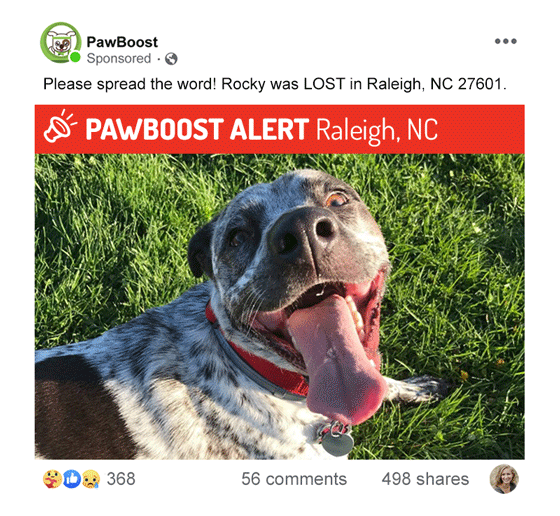
\includegraphics[scale=0.5]{slike/pawBoost.PNG} 
			\centering
			\caption{oglas platforme PawBoost}
			\label{pawBoost}
		\end{figure}
		
		\begin{figure}[H]
			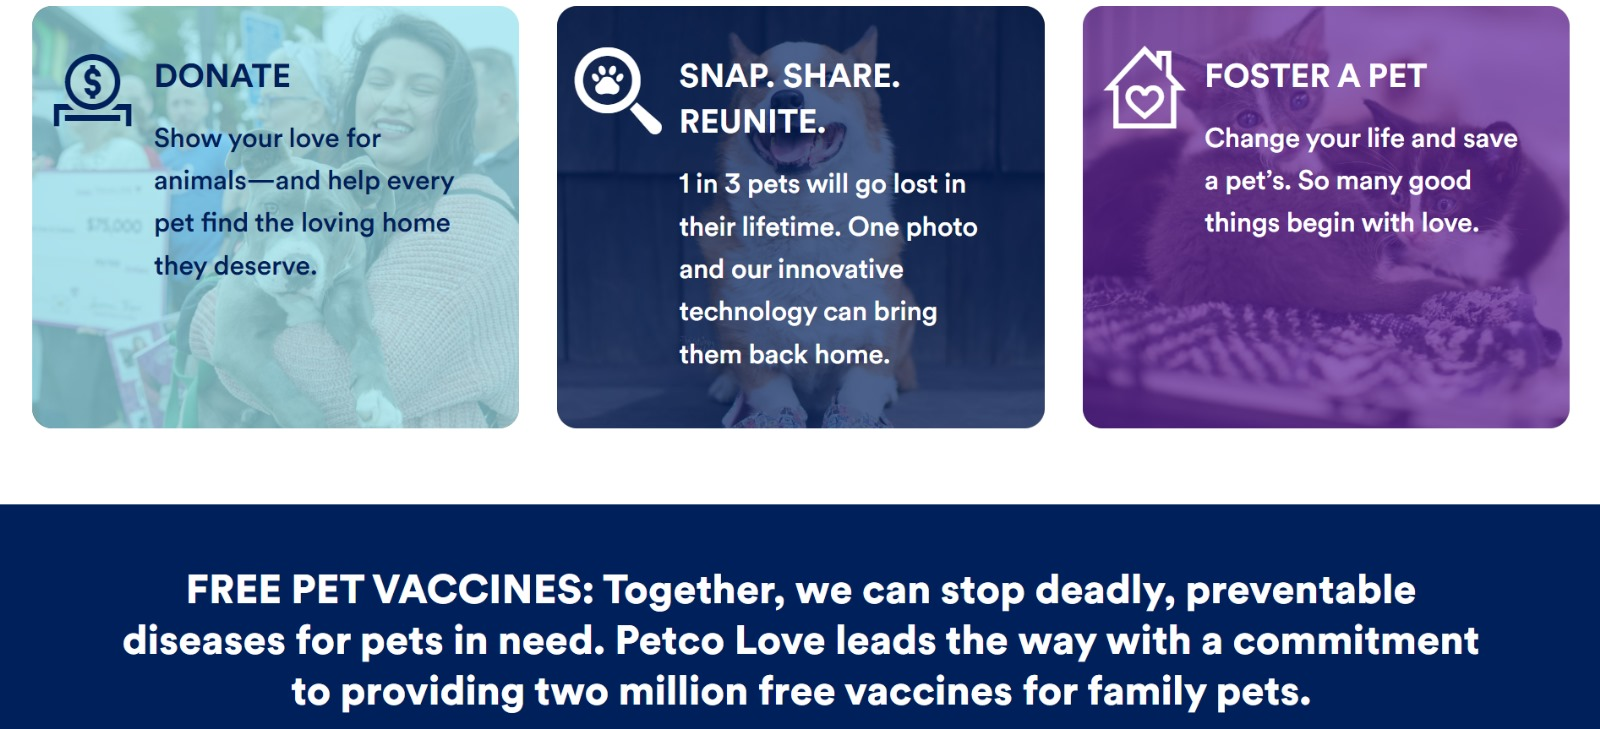
\includegraphics[scale = 0.4]{slike/petcoLove.PNG} 
			\centering
			\caption{usluge koje nudi platforma PetcoLove}
			\label{petcoLove}
		\end{figure}
		
		\begin{figure}[H]
			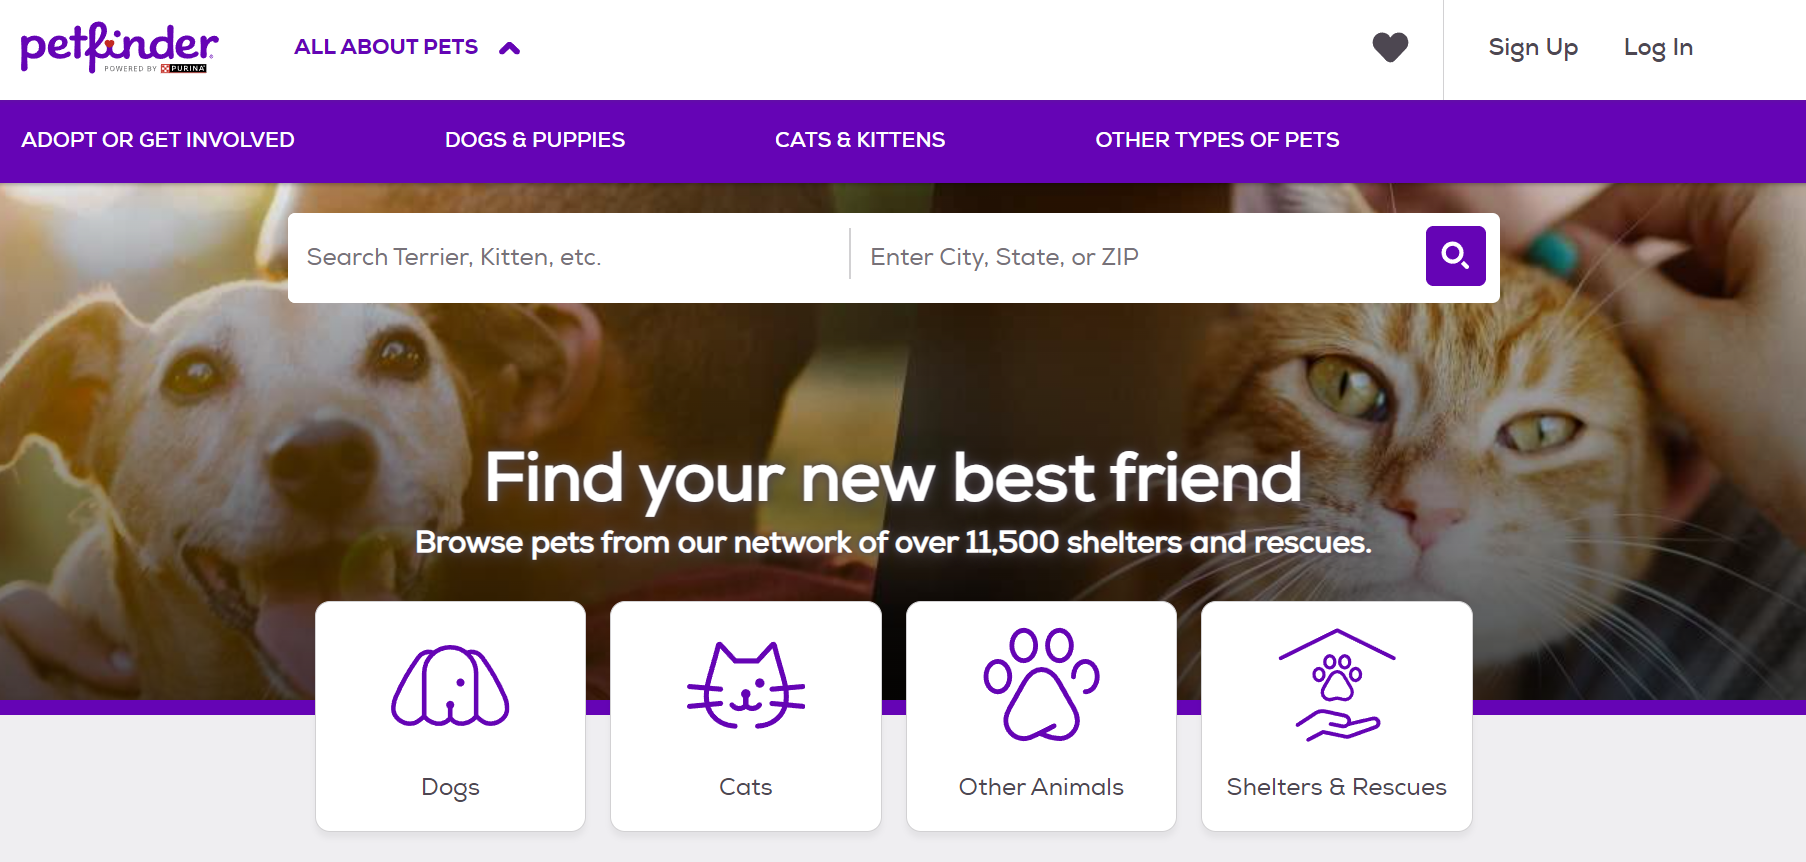
\includegraphics[scale = 0.5]{slike/petFinder.PNG} 
			\centering
			\caption{web stranica platforme PetFinder}
			\label{petcoLove}
		\end{figure}
		
		\pagebreak
		
		
		\section{\textbf{Moguće prilagodbe i nadogradnje rješenja}}
		
		\begin{packed_item}
		
			\item Lokaliziranjem aplikacije ona bi postala dostupna i korisnicima u zemljama s drugim jezicima, zakonima i običajima.
			
			\item Osnovni princip naše aplikacije se može primijeniti i na razne izgubljene predmete. Naša aplikacija je svojevrsni \textit{lost and found}(rekonstrukcija nestanka) primijenjen na ljubimce.
			
			\item Nakon početne implementacije, neke od mogućih projektnih nadogradnji uključuju i \textit{real time chat} opciju. Korisnici mogu međusobno privatno komunicirati i dijeliti razne informacije o nestalim ljubimcima. Registrirani korisnik s informacijama koje mogu pomoći vlasniku izgubljenog ljubimca može kontaktirati dotičnog vlasnika koji je objavio oglas.
			
			\item Uvođenje naprednih algoritama za prepoznavanje životinja putem fotografija olakšalo bi i ubrzalo pronalazak.
			
			\item Povezivanjem podataka veterinarskih klinika i baze prijavljenih životinja aplikacije može doći do preklapanja upita u bazi podataka. Time bi se napravio korak dalje u zbližavanju vlasnika i nestalog ljubimca.
			
			\item Na web aplikaciji bi mogla postojati mogućnost donacije sredstava lokalnim skloništima za životinje.\\
			
		\end{packed_item}
		
		Web aplikacija je namijenjena za 3 vrste korisnika; neregistriranom korisniku, registriranom te skloništima za životinje (specijalni tip registriranog korisnika).\\
		
		\textbf{Neregistrirani korisnik} ima mogućnost pregledavanja i pretraživanja nestalih kućnih ljubimaca. Klikom na sliku nestale životinje, znatiželjnom korisniku otvaraju se informacije o njoj: vrsta, ime, datum i sat nestanka, lokacija nestanka, boja, starost, tekstni opis. Uz to dostupne su do 3 slike te životinje kako bi ju tragač lakše pronašao, a ako bi došlo do novih informacija ili pronalaska ljubimca dostupni su i kontakt podaci vlasnika. Neregistrirani korisnik bi se trebao registrirati ako bi poželio sudjelovati u potrazi i ostvariti komunikaciju s dotičnim vlasnikom.\\
		
		Za registraciju je potrebno ostaviti određene osobne podatke:
		
		\begin{packed_item}
			\item Elektronsku poštu
			\item Broj telefona
			\item Naziv skloništa (opcionalno)
		\end{packed_item}
		
		\textbf{Registrirani korisnik} ima širi spektar mogućnosti unutar aplikacije. On može, uz pregledavanje i pretraživanje, postaviti oglas o nestalom ljubimcu, izmijeniti i ukloniti ga pa i sudjelovati u komunikaciji s drugim registriranim korisnicima.\\
		
		Postoje 4 kategorije oglasa:
		
		\begin{packed_item}
			\item Za ljubimcem se traga (početna postavka oglasa)
			\item Ljubimac je sretno pronađen
			\item Ljubimac nije nađen, ali se ne traga aktivno
			\item Ljubimac je pronađen pod nesretnim okolnostima
		\end{packed_item}
		
		\textbf{Skloništa za životinje} su vrsta registriranih korisnika koji oglašavaju životinje koje su pronašli te se nalaze kod njih.\\\\
		
		

		U nastavku se nalaze različiti primjeri kako koristiti osnovne funkcionalnosti \LaTeX a koje su potrebne za izradu dokumentacije. Za dodatnu pomoć obratiti se asistentu na projektu ili potražiti upute na sljedećim web sjedištima:
		\begin{itemize}
			\item Upute za izradu diplomskog rada u \LaTeX u - \url{https://www.fer.unizg.hr/_download/repository/LaTeX-upute.pdf}
			\item \LaTeX\ projekt - \url{https://www.latex-project.org/help/}
			\item StackExchange za Tex - \url{https://tex.stackexchange.com/}\\
		
		\end{itemize} 	


		
		\noindent \underbar{podcrtani tekst}, \textbf{podebljani tekst}, 	\textit{nagnuti tekst}\\
		\noindent \normalsize primjer \large primjer \Large primjer \LARGE {primjer} \huge {primjer} \Huge primjer \normalsize
				
		\begin{packed_item}
			
			\item  primjer
			\item  primjer
			\item  primjer
			\item[] \begin{packed_enum}
				\item primjer
				\item[] \begin{packed_enum}
					\item[1.a] primjer
					\item[b] primjer
				\end{packed_enum}
				\item primjer
			\end{packed_enum}
			
		\end{packed_item}
		
		\noindent primjer url-a: \url{https://www.fer.unizg.hr/predmet/proinz/projekt}
		
		\noindent posebni znakovi: \# \$ \% \& \{ \} \_ 
		$|$ $<$ $>$ 
		\^{} 
		\~{} 
		$\backslash$ 
		
		
		\begin{longtblr}[
			label=none,
			entry=none
			]{
				width = \textwidth,
				colspec={|X[8,l]|X[8, l]|X[16, l]|}, 
				rowhead = 1,
			} %definicija širine tablice, širine stupaca, poravnanje i broja redaka naslova tablice
			\hline \SetCell[c=3]{c}{\textbf{naslov unutar tablice}}	 \\ \hline[3pt]
			\SetCell{LightGreen}IDKorisnik & INT	&  	Lorem ipsum dolor sit amet, consectetur adipiscing elit, sed do eiusmod  	\\ \hline
			korisnickoIme	& VARCHAR &   	\\ \hline 
			email & VARCHAR &   \\ \hline 
			ime & VARCHAR	&  		\\ \hline 
			\SetCell{LightBlue} primjer	& VARCHAR &   	\\ \hline 
		\end{longtblr}
		

		\begin{longtblr}[
				caption = {Naslov s referencom izvan tablice},
				entry = {Short Caption},
			]{
				width = \textwidth, 
				colspec = {|X[8,l]|X[8,l]|X[16,l]|}, 
				rowhead = 1,
			}
			\hline
			\SetCell{LightGreen}IDKorisnik & INT	&  	Lorem ipsum dolor sit amet, consectetur adipiscing elit, sed do eiusmod  	\\ \hline
			korisnickoIme	& VARCHAR &   	\\ \hline 
			email & VARCHAR &   \\ \hline 
			ime & VARCHAR	&  		\\ \hline 
			\SetCell{LightBlue} primjer	& VARCHAR &   	\\ \hline 
		\end{longtblr}
	


		
		
		%unos slike
		\begin{figure}[H]
			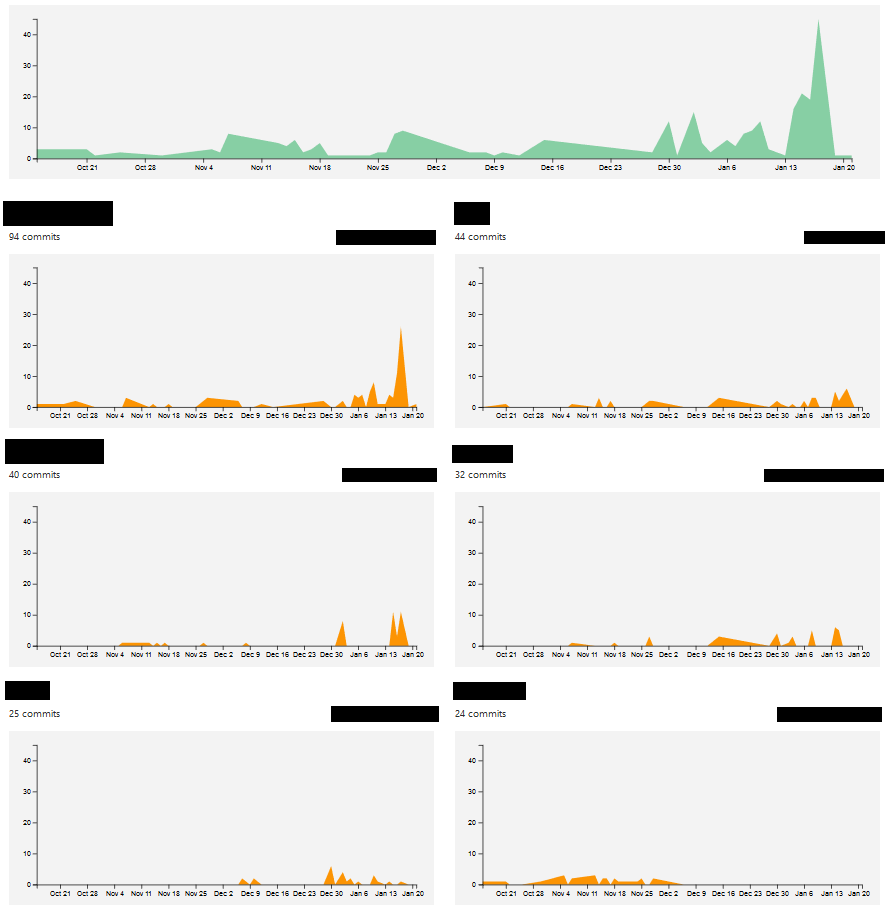
\includegraphics[scale=0.4]{slike/aktivnost.PNG} %veličina slike u odnosu na originalnu datoteku i pozicija slike
			\centering
			\caption{Primjer slike s potpisom}
			\label{fig:promjene}
		\end{figure}
		
		\begin{figure}[H]
			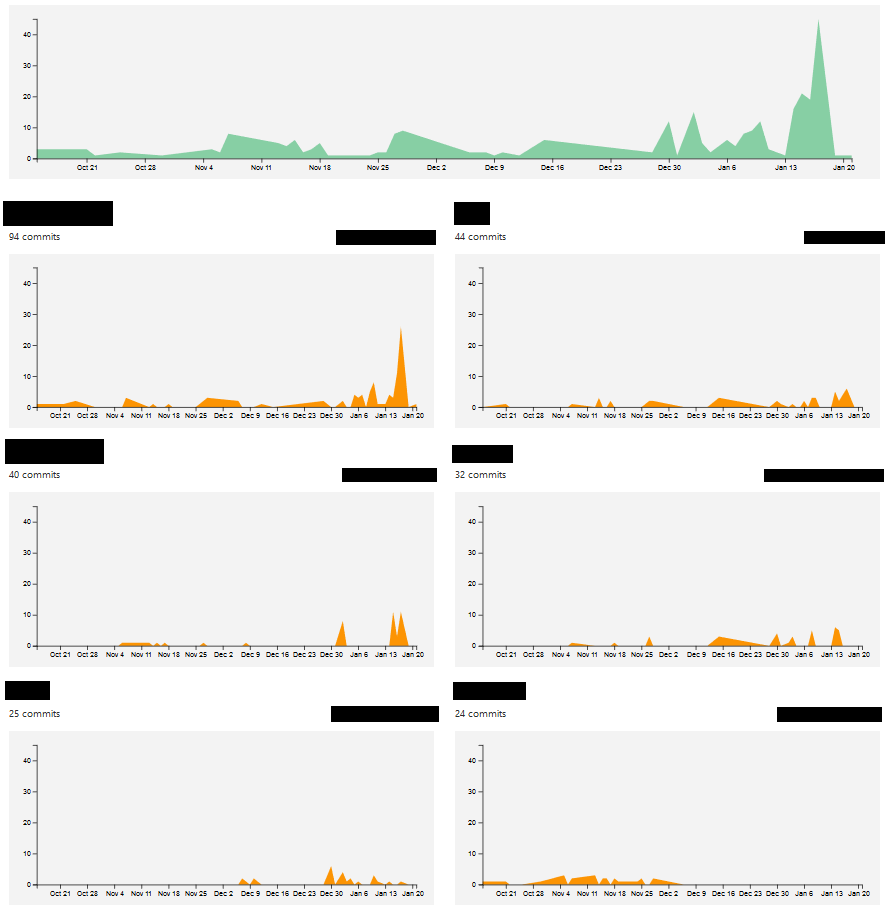
\includegraphics[width=\textwidth]{slike/aktivnost.PNG} %veličina u odnosu na širinu linije
			\caption{Primjer slike s potpisom 2}
			\label{fig:promjene2} %label mora biti drugaciji za svaku sliku
		\end{figure}
		
		Referenciranje slike \ref{fig:promjene2} u tekstu.
		
		\eject
		
	